\chapter{Literature Survey}

This section will explain why there’s a need for this system by exploring background literature related to this subject. Mainly the need of a proper system to test scientific software, start with explaining what a scientific software is, following up by explaining why most of them are not tested correctly. Then we will be discussing some of the current method in testing and why are they insufficient. Next we will be discussing the two main components of this system, Cucumber and Behave. Then finally, explaining what casual testing is, the main method used by this system to test other software, and exhibit why it lacks a proper interactive system for non software engineering users. 

\section{Computational models}
Using a computational model for scientific research is common practice with today’s technology, scientists use these models to predict the result of an experiment or the outcome of an event. But whether these models can accurately predict the result, is still a problem since most of them lack some form of proper testing. Below will be discussing what is a computational model, why they are poorly tested, and some of the current testing method.

\subsection{Introduction to computational model}
Computational model use computers to simulate and study real life events by using mathematics, statistics, physics, and computer science to study the mechanism and behavior of complex systems by computer simulation \cite{Reference1}. There are two main ways to process model’s data, empirical and mechanistic, each have its own benefits. \\*\\*
For empirical, researcher don’t need to know exactly how the system works, they just need to observe the outcome of certain scenario and predict what’s going to happen in the future \cite{Reference5}. For example, by observing how tides are going to change in a year, people can predict how the tides will change in the upcoming years. They don’t need to know the exact mechanism behind why and how the tides change, only require knowing the circumstance and the outcome. By using this method, it simplifies the model since there’s less complex calculation required. And it’s better to comprehend compared to mechanistic. The problem for empirical is it require a lot more input data to have good accuracy in the model, there won’t be much problem if the model is developed with big data and machine learning tools, but if the model don’t have enough data at the start, it will affect the model’s accuracy. \\*\\*
For mechanistic, it requires fewer input data to achieve the same accuracy as the empirical, but it is also more computationally intensive\cite{Reference5}. Compared to empirical, it is easier to extrapolation, researchers can make predictions based on the previous input data. \\*\\*
In terms of the implementation of model, it is split into two types, agent based and equation-based model. \\*\\* 
For agent-based model, is a system is modeled as a collection of autonomous decision-making entities called agents. Agents will act based on the situation its in and the abilities it has \cite{Reference6}. Agents with react appropriate to the rule defined for them, for example, in an agent-based model for honeybee, if a bee detect a flower near by with resource in it, the bee will move toward the flower and collect the resource. In this case, the bee agent is in a situation where there is flower with resource nearby, according to the rules define for the bee agent, it reacts by moving towards the flower and collect from it. \\*\\*
For equation-based model, instead of have agents with rules defined, it have a set of differential equations, the model uses equations to represent relationships between observables \cite{Reference7}, the situation of observables will change depend on the equation. For example, modeler can define an equation on how fast a disease will spread, by define a start infected population, the equation can then calculate how many people are infected in each given timestep. \\*\\*

\subsection{Purpose of computational model}
By using models that contain a number of input variables, and algorithms that will define the system. Researchers use these models to simulate real-life situations and adjust these models by changing their variable and algorithm according to the results to make the model more conform to reality. Then researchers can use these models to see how one or more variables can affect the outcome of a certain event. Computational models provided some level of prediction of being able to calculate an anticipated result from a given set of variables \cite{Reference8}. This forecasting system can be used to predict complex systems, such as weather or disease spread, and help researchers or decision makers to decide their next move.\\*\\*
An example of this kind of model is Covasim \cite{Reference9}, this model is used heavily in the implementation of Causcumber, a tool for testing in computational model that will discuss later. Covasim uses agents to simulate individual people, the model mainly focused on one type of calculation, what is the probability of an individual in a given time step will change from not infected to infected, or badly ill to death. \\*\\*
The simulation starts from loaded the parameters, then it will start creating individual with different age, sex, and comorbidities based on the selected location (i.e., Different country). Then agents will be grouped into a social network depending on their attributes. After that the model will start looping, in each step, the model will apply various operations on the individual, then collect the result and apply analysis.

\section{Testing computational models}
Computational models are often very complicated, and require special knowledge related to the field, so is testing computational model. This often results in some issue in testing, some methods have been developed to help with the testing process, but most are either to complicate or insufficient. There’s currently a more efficient way to test these models which is by using behavior-driven development (or BDD) and Cucumber. Combined with casual model testing, a way to draw relationships between variables, it will make testing these complex models a lot easier.

\subsection{Why computational models are hard to test}
Computational models are often developed by scientists themselves, but most scientists aren’t software developers and may not have knowledge in some common software engineering practices, this may cost the quality of the scientific software \cite{Reference10}. Software testing is one of the aspects that is impacted, since the lack of knowledge in software development, lack of understanding in systematic testing is expected. Mistake can be made without notice and may affect the output of the system, causing the result to become inaccurate.\\*\\*
Testing a scientific software itself can be a difficult task to do, this may be the result of two types of challenges: \\*\\*
First is due to the software’s main purpose is to predict something unknown or simulate areas even researchers have little knowledge in, but to test a software, it is crucial to know how the software should behave, what kind of output should it show. Without these knowledge, it is hard to tell if the software is working the right way. Furthermore, these computation models are often consisting of hundreds of parameters and complex algorithm, this means it would require lots of test case in order to test every aspect of the system, and this leads high execution time making the testing process become very time consuming \cite{Reference10}.\\*\\*
Second is that scientific software is mostly developed with scientists being the lead role instead of a software engineer, and the value of the software system is often underestimated \cite{Reference10}. And most scientists never went through the training in software design like software engineer \cite{Reference11}, this means limited understanding of the testing process and not applying known testing methods. This will make the core design of the software unfriendly for effective testing.

\subsection{Current testing methods and its disadvantage}
After modeler complete the modeling process, they are required to verify the model. 
Despite the rarely carried out practice, verification is an important step in modeling, it helps making sure the results produced by the model is accurate enough to represent the reality or the theory of the model. Verification is done by comparing the predication of the model with actual data. The type of compared data provide will determine whether the models is validated at the pattern, point, distribution, or value level, or some combination of these \cite{Reference12}. \\*\\*
This verification step can have some issue when it comes to models with multiple agents, modelers may be required to test the agent as an individual or in as a group, this is often determined by the requirement of the model. If the model’s main goal is focus on the broader environment, then its agents need to be verified as a group\cite{Reference12}. For example in a model for researching bee colony’s behavior, the bee agents will be assessed as an entire hive instead of as individual bees. On the contrast, if the model’s goal is focus on individual agent, it will need to be verify as an individual.
The modelers will be required to collect data to compare it with the results of the model. This can make the verification process become very tedious and time consuming. 

\section{Advanced testing techniques for computational models}
With the drawback of the current testing method, more advanced method is developed to make testing more efficient. But this isn’t without any issue, advance method require tester to have specific knowledge in software testing, which is not common for scientist developed the computational model.

\subsection{Behavior-driven Development with Behave}
Behave is a python API based on behavior-driven development, where the goal is for people who don’t really understand programming code to be able to participate in the testing process. Behavior-driven development is a development technique that encourages collaboration between participants in a software project \cite{Reference13}. Behavior-driven development or BDD, aims to have a clear understanding of the desired software behavior between stakeholders and software developers, and communicate by writing test cases in a natural language that both sides can understand. Behave is a Python API created for this, it consists of tests written in Cucumber, another API written in natural language style. \\*\\*
When a test case is written, it requires a tool to read its specifications and see if the system works as the test-case specified. Cucumber is the tool that was developed for this purpose, it reads specifications written in plain text with a certain format and validates if the software does what those specifications say \cite{Reference14} and creates a report. \\*\\*
For the non-developers who want to participate in testing, they are required to create a feature file. The feature need be written in Gherkin language, Gherkin uses a set of grammar and special keywords to give plain text structure so that Cucumber could understand it, one of the pros for Gherkin is that keyword can be translated to other languages, making it usable for people who don’t speak English \cite{Reference15}. A proper Gherkin grammar starts by giving a context, then describing an event, and after that what should happen after the event. With these grammars, testers can specify a situation in the system, describe a certain parameter, and what the results should be with those parameters. By writing a test using Cucumber and Gherkin grammar, tester can combine them into a .Feature file as display below: 
\begin{figure}[h]
	\centering
	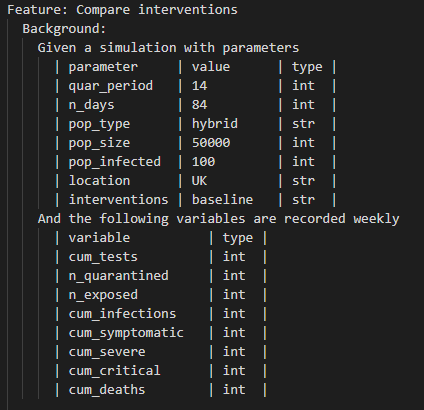
\includegraphics[width=10cm]{figures/featureFile.png}\\
	\caption{A feature file example.}
	\label{fig:figure1}
\end{figure}
\newpage \noindent 
\\*\\*
For developers, they are required to create a step decorator the matches the steps, for example in the above feature file example, there is a “given” type, therefore in step decorator will need to match it as below:
\begin{figure}[H]
	\centering
	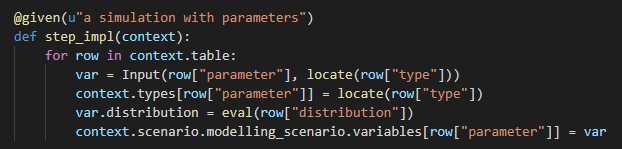
\includegraphics[width=10cm]{figures/stepFile.png}\\
	\caption{A step decorator example.}
	\label{fig:figure2}
\end{figure}
\noindent 
With the step file implemented, tester can execute the .feature file in terminal and Behave can read what needs to be tested and return a report. In this way, tester who don’t have sufficient knowledge can involve in testing phase, therefore making collaboration between developers and non-developer in a project become a lot easier.

\subsection{Causal testing}
With the help of Behave and Cucumber, we have the ability to test computational models. It is possible to test the entire system by writing an enormous feature file, but the execution time will become really long, and since computational models are usually in big scale it is also easy to make mistakes. This is when causal model can help simplify the testing process. \\*\\*
Causal model is a way to represent causal relationship within a system through mathematical model. It helps testers monitor causal relationships in the data \cite{Reference16}. A causal module can predict the behavior of a system, by comparing different inputs and the outputs a system produces, it can explore the cause and influence of a certain relationship \cite{Reference17}. Tester can purposefully change a certain input to observe the change in behaviour, when change in input cause change in output, tester can observe causal relationship between the variables. When there’s a difference between in executions of the system, whether its in input or the execution process, no matter how small it is, these differences can help testers identify any unusual behaviour in the system.\cite{Reference18} \\*\\*
With this method testers can reduce the time required to test a complicated system by only testing parts of it one at a time, then combine the results, and testers can have a full picture of how the system performs. This is unlike the traditional method, where it requires testing the entire system all at once, and may require lots of time if it is a complicated system. \\*\\*

\subsection{Testing computational model with causal testing}
Despite the existing implementation of combining Behave and causal testing, Causcumber, it still requires more assist in order to make this system more easy to approach. Causal testing can be a really useful testing method for software engineers \cite{Reference19}, however computational models are often developed by scientists or researchers who have limited knowledge in software testing \cite{Reference13}. Tester who wants to use causal model to test system needs to have prior knowledge in how variables work in a software, this means people who may not have that much knowledge in software engineering, for example researchers in other fields, might not be able to conduct this method of testing in their software. \\*\\*
Causcumber is a system incorporate Behave and Cucumber into Causal testing, testing with Causal testing become more accessible for people who don’t have specific knowledge in software testing. Without Behave, testers will need to either design inputs them self or using auto test value generation \cite{Reference12}, but either option will require testers to have sufficient training in software testing, which are not common among scientists or researchers who developed computational model. And with Behave, user can specify the testing cases in a more natural language, making creating testing case more accessible. After creating test case for computational model, user can compare different test cases to identify the behaviour of the system and use the behaviour to identify if the subject system is behaving correctly.\\*\\*
But in the current version of Cucumber, it requires users to edit the test case file directly, which still require user to use a certain syntax to make sure the test cases work with the decorator. There’s still a need to further streamline this process, to achieve this, we can implement a GUI to guild and assist tester to in the testing process. With this GUI, tester can use it to create test case without the need to interact with the coding part of the system. This approach can make the testing process even more accessible.


\section{Summary}
Testing a computational model isn’t a easy task, not only because there can be lots of unknowns in the developing of computational model, but also because among the people who develop those software, most have limit experience in software testing. The current testing method is by gather lots of data and compare those data with the result produced by the model, this method may be useful, but can become tedious with more complex model. To make this process more convenient, several tools can be used to help simplify the process. With Behave, an API based on the behavior-driven development method, tester can specify the test case in a natural language, making test process a more approachable, encouraging people who do not specialize in software engineering to take part in testing. With causal model, testers can effectively test large and complex computational models. By using different test cases, tester can compare the inputs, outputs and the execution path of the test cases to identify the behaviour of the system. And with the behaviour, tester can verify if the software is working as intended. But the problem is that when using causal model testing, it is inaccessible for most people, due to its requirement for user to have knowledge in software testing. To make it more user friendly, Behave is integrated to make it where users can create test case with a relatively natural language. But it still require a certain syntax to work, so a way to further simplify the testing process is needed, which leads to the development of a GUI to help streamline this process.
